\documentclass{article}
\usepackage[utf8]{inputenc}
\usepackage[usenames,dvipsnames]{xcolor}
\usepackage{pdfpages}	  % Insertion of PDF-pages

% Sideopsætning
\usepackage{geometry}                       % Håndtering af papirstørrelse og marginer
\geometry{a4paper, twoside}                 % Papirstørrelse
\geometry{top=2.5cm, bottom=2.5cm}		    % Øvre og nedre margin
\geometry{left=2.5cm, right=2.5cm}		    % Venstre og højre margin

% Tekstformatering
\setlength{\parindent}{0pt}				    % Indryk
\linespread{1.2}							% Linjeafstand
\usepackage[dvipsnames]{xcolor, colortbl}	% Farvekommandoer
\newcommand{\myparagraph}[1]{\paragraph{#1}\mbox{}\\} % Paragraph med newline efter

\begin{document}

\title{IsLeapYear algorithm diagram}
\author{Rebekka Viktoria Mejlhede Eriksen}
\maketitle
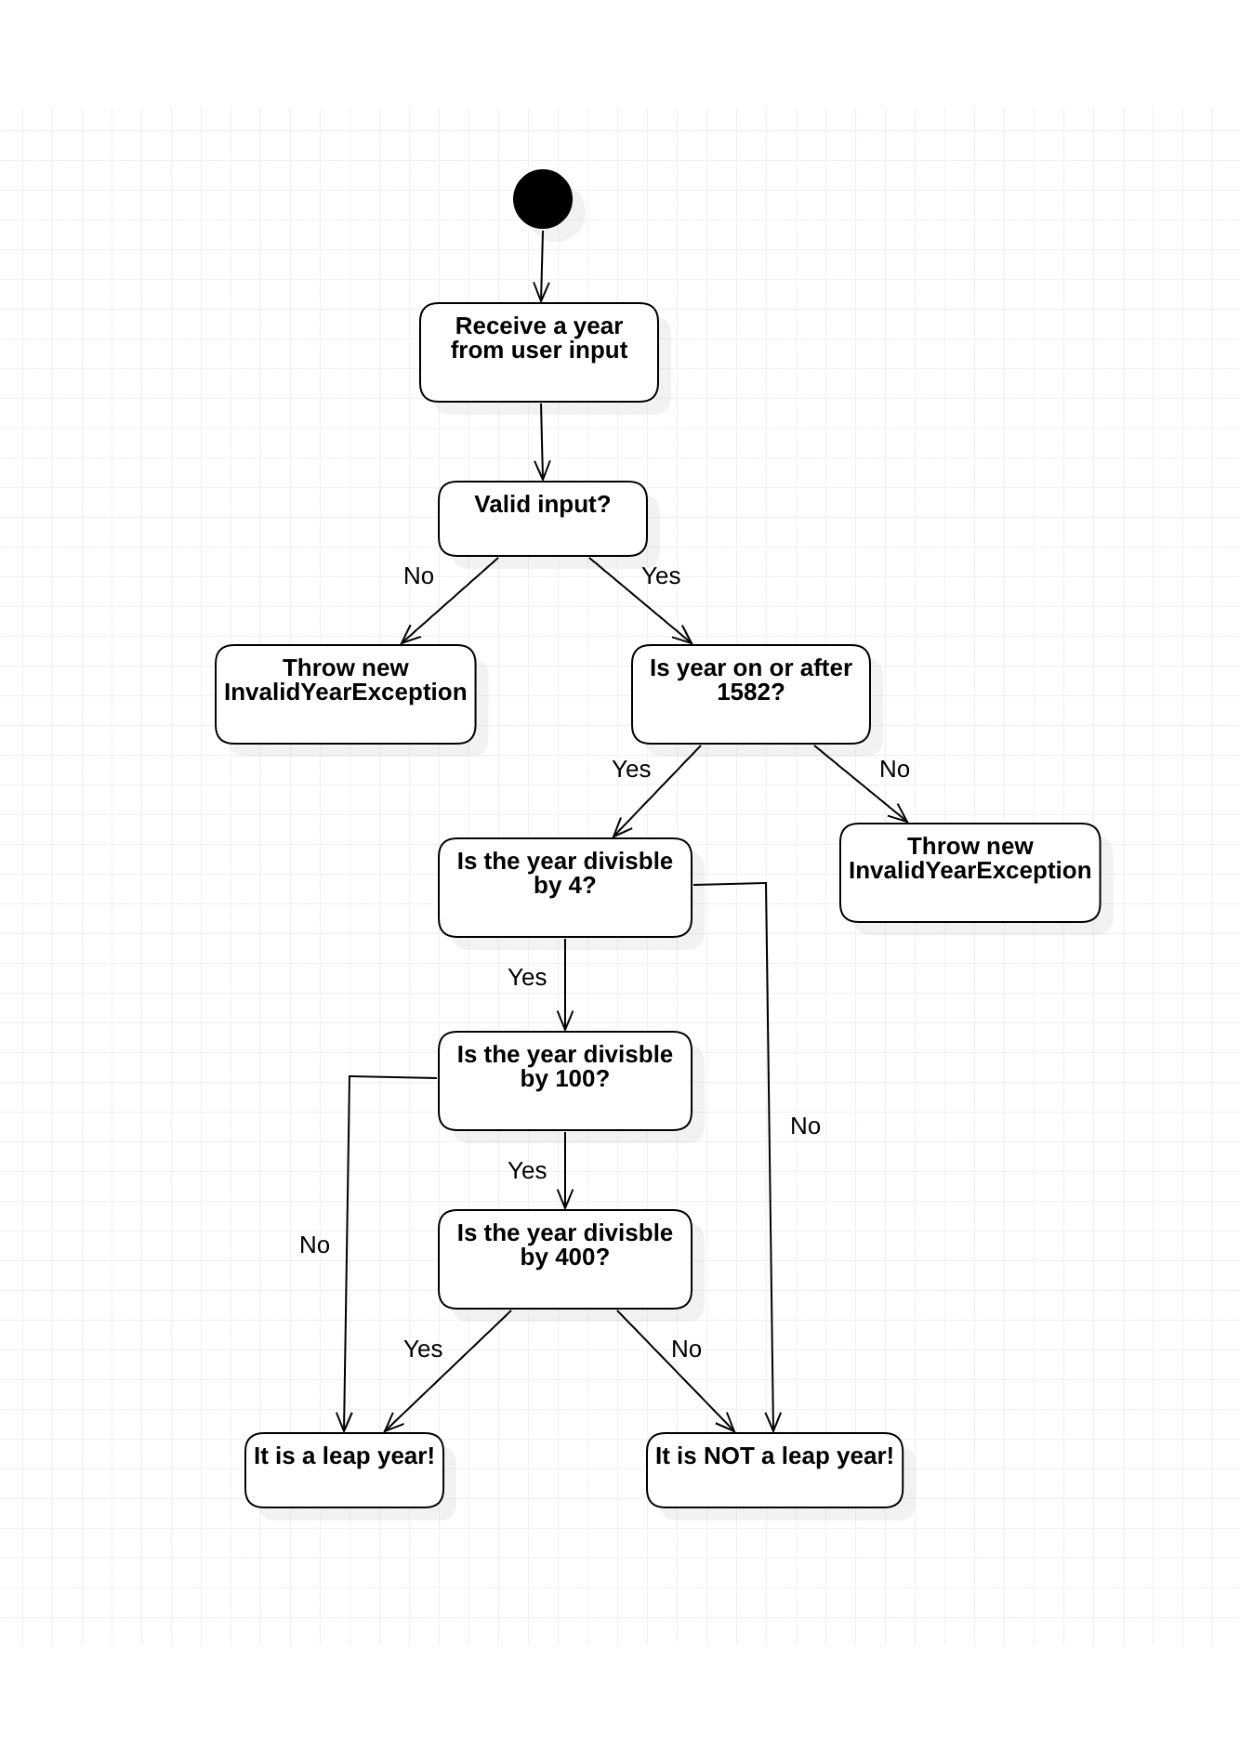
\includepdf[pages=-]{Diagrams/LeapYearUML.pdf}
\newpage

This diagram shows how the program acts when executed.

\end{document}